\documentclass[11pt]{article}
\usepackage[margin=0.82in]{geometry}
\usepackage{graphicx,booktabs,amsmath,amssymb,array,microtype,url,hyperref,xcolor,float}
\usepackage[font=small,labelfont=bf,skip=7pt]{caption}
\setlength{\parindent}{1.25em}
\setlength{\parskip}{0.15em}
\setlength{\textfloatsep}{14pt plus 2pt minus 2pt}
\setlength{\floatsep}{12pt plus 2pt minus 2pt}
\hypersetup{colorlinks=true,linkcolor=black,citecolor=blue,urlcolor=blue}
\title{Leakage-Aware E-Commerce Churn Prediction with Extremely Randomized Trees and Grouped Evaluation}
\author{Anonymous Author\\Affiliation withheld for review}
\date{}
\begin{document}
\maketitle
\begin{abstract}
Customer churn models for e-commerce must identify a rare positive class without obtaining high accuracy by predicting retention. We evaluate this problem on a cleaned snapshot of 5,630 customers containing 948 churners (16.84\%) and 18 candidate predictors. Identical predictor profiles were assigned to the same group, producing 5,071 groups; all preprocessing, feature selection, sampling, hyperparameter search, calibration, and threshold choice were confined to development folds. Five-fold grouped out-of-fold evaluation compared logistic regression, decision trees, Random Forest, Extra Trees, XGBoost, LightGBM, CatBoost, engineered behavioral features, class weighting, random oversampling, SMOTE, feature selectors, calibration, and probability blending. A fixed 20\% group-aware holdout was evaluated once after selection. The selected Extra Trees model used all 18 predictors and a development-selected threshold of 0.45. On 1,126 locked-test customers it achieved 97.25\% accuracy, 94.89\% precision, 88.36\% recall, 0.9151 F1, 0.9747 average precision, and 0.9938 ROC-AUC, with TN=928, FP=9, FN=22, and TP=167. Against a newly executed 12-feature oversampled Random Forest on the identical records, paired bootstrap differences favored Extra Trees by 0.0612 F1 (95\% CI 0.0326--0.0931) and 0.0230 average precision (0.0112--0.0376). Published results from Sun (2025) are reported descriptively because their split and one-record-smaller dataset differ. The principal contribution is an auditable, group-preserving evaluation showing that randomized tree ensembles improved both overall performance and churn detection without test-label optimization.
\end{abstract}

\section{Introduction}
Customer attrition reduces recurring revenue and increases acquisition pressure. In e-commerce, the operational goal is rarely to maximize accuracy alone: when only 16.84\% of customers churn, a trivial retention prediction is already 83.16\% accurate. A useful system must preserve precision while recovering a large fraction of churners and producing risk scores suitable for constrained outreach.

Prior work applied logistic regression, decision trees, and XGBoost with oversampling to this dataset family \cite{sun2025churn}. The published study emphasized XGBoost's ROC-AUC of 0.9667, although its decision tree had higher accuracy and F1. That result motivates stronger evaluation rather than a presumption that one boosting algorithm dominates. Repeated customer profiles and uncertainty about the cleaned workbook's preprocessing lineage create additional leakage risks.

This study asks three questions: (RQ1) which learner provides the best balance of accuracy, churn recall, F1, and average precision on identical group-held-out observations; (RQ2) do paper-derived and behavior-based features, imbalance handling, selection, calibration, or blending add value under nested controls; and (RQ3) is any observed gain paired and statistically defensible? Our contributions are: a deterministic profile-group protocol; controlled E0--E8 experiments spanning strong tree ensembles and ablations; OOF-only threshold selection with an accuracy floor; and paired uncertainty estimates on a locked holdout. Figure~\ref{fig:method} summarizes the design.

\begin{figure}[H]
\centering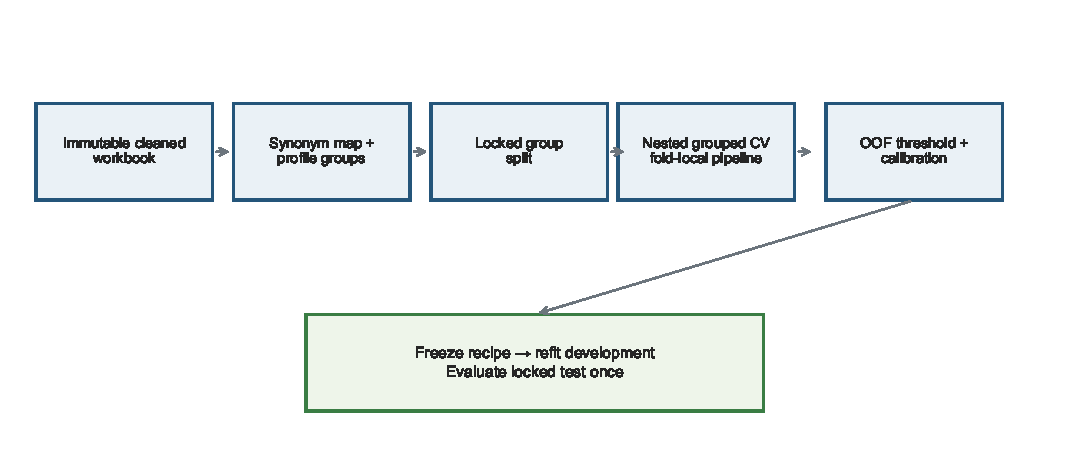
\includegraphics[width=.88\textwidth]{figures/fig01_methodology.pdf}
\caption{Leakage-aware experimental architecture. The final test partition is downstream of every modeling decision.}\label{fig:method}
\end{figure}

\section{Related Work}
Random Forest combines randomized tree predictors and connects performance to individual-tree strength and correlation \cite{breiman2001rf}. Extra Trees extends randomization to split-point construction \cite{geurts2006extra}. XGBoost introduced sparsity-aware scalable boosting \cite{chen2016xgb}; LightGBM proposed gradient-based one-side sampling and exclusive feature bundling \cite{ke2017lgbm}; and CatBoost addressed prediction shift and categorical target-statistic leakage through ordered learning \cite{prokhorenkova2018cat}. SMOTE synthesizes minority-class neighbors \cite{chawla2002smote}, but sampling must remain inside training folds. Probability calibration can use sigmoid or isotonic mappings \cite{niculescu2005calibration}. Model explanations can use SHAP values \cite{lundberg2017shap}; here permutation importance was chosen because it directly measures held-development score degradation without claiming causal effects.

\begin{table}[H]\centering\small\setlength{\tabcolsep}{6pt}
\caption{Selected methodological literature.}\label{tab:lit}
\begin{tabular}{p{2.6cm}p{3.0cm}p{10.0cm}}\toprule
Work & Data/approach & Relevance and limitation \\\midrule
Breiman (2001) & Random forests & Ensemble foundation; not churn-specific.\\
Geurts et al. (2006) & Extra Trees & Randomized cut points; winning family here.\\
Chen and Guestrin (2016) & XGBoost & Scalable boosting; compared under identical folds.\\
Ke et al. (2017) & LightGBM & Efficient GBDT; used for ablations.\\
Prokhorenkova et al. (2018) & CatBoost & Ordered boosting; categorical method not used natively because learners shared one-hot inputs.\\
Sun (2025) & 5,629 e-commerce rows & Closest study; protocol differs from this work.\\
\bottomrule\end{tabular}
\end{table}

\section{Dataset and Exploratory Analysis}
The modeling source is the workbook's \texttt{Cleaned Data} sheet: 5,630 rows, 20 columns, unique \texttt{CustomerID}, binary \texttt{Churn}, and 18 predictors. It contains 4,682 retained customers and 948 churners, no missing cells, no duplicate customer identifiers, and no full-row duplicates. The paper reports 5,629 observations, so the versions cannot be asserted identical. We retained all legitimate workbook rows.

Two fixed synonym mappings were applied: \texttt{Phone} to \texttt{Mobile Phone} for login device (1,231 rows), and \texttt{Mobile} to \texttt{Mobile Phone} for preferred category (809 rows). These deterministic business-synonym transformations do not use labels. Hashing all standardized predictors yielded 5,071 profiles, including 559 repeated groups covering 1,118 rows and no conflicting-label groups. Grouping prevents identical profiles from crossing evaluation boundaries.

\begin{table}[H]\centering\scriptsize\setlength{\tabcolsep}{4pt}
\caption{Dataset characteristics and audit.}\label{tab:data}
\begin{tabular}{lr}\toprule
Item & Value\\\midrule
Customers / predictors & 5,630 / 18\\
Churn / stay & 948 / 4,682\\
Churn prevalence & 16.84\%\\
Missing cells / duplicate IDs & 0 / 0\\
Profile groups & 5,071\\
Repeated groups / rows & 559 / 1,118\\
Conflicting-label groups & 0\\
Development / locked test & 4,504 / 1,126\\
SHA-256 prefix & \texttt{371acba4a77fc4e6}\\
\bottomrule\end{tabular}
\end{table}

Figure~\ref{fig:balance} shows the imbalance. Figure~\ref{fig:corr} provides a Spearman association view for numeric variables; it is exploratory and does not justify causal claims.
\begin{figure}[H]\centering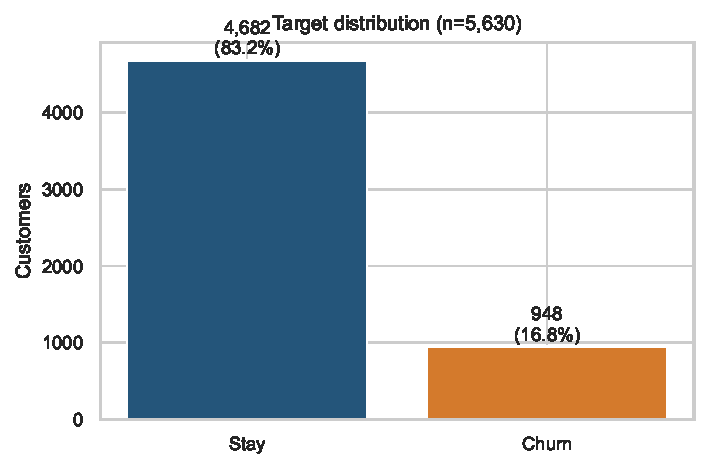
\includegraphics[width=.58\textwidth]{figures/fig02_class_balance.pdf}\caption{Class distribution in the cleaned workbook.}\label{fig:balance}\end{figure}
\begin{figure}[H]\centering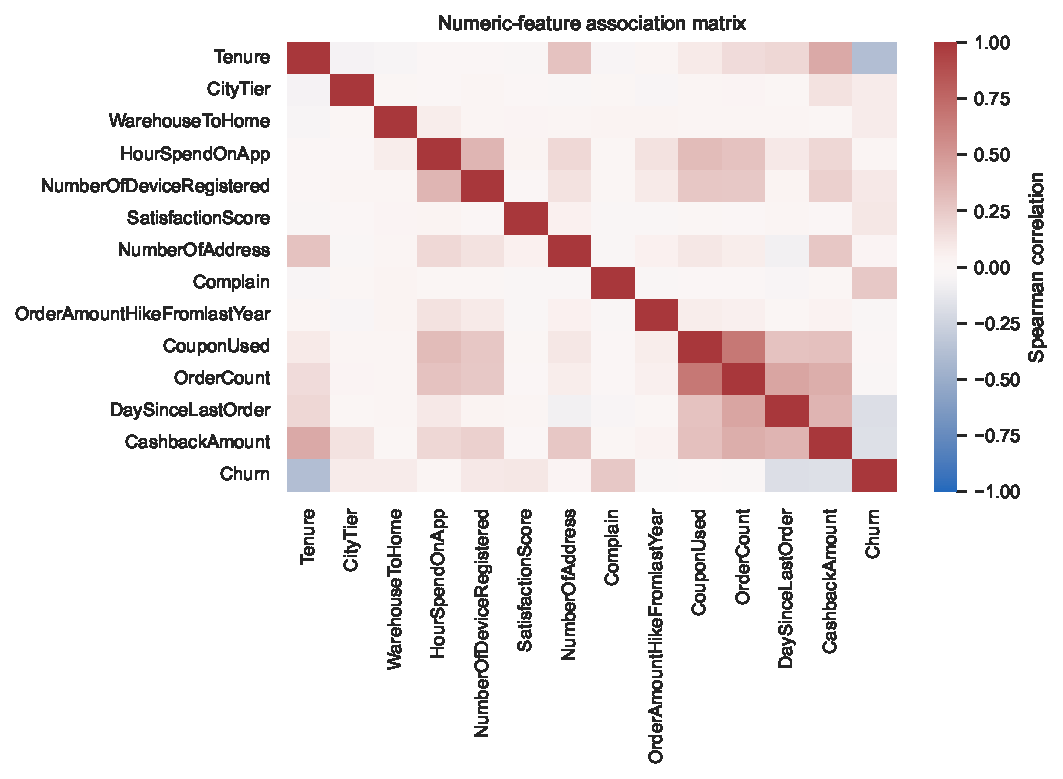
\includegraphics[width=.78\textwidth]{figures/fig03_feature_association.pdf}\caption{Numeric-feature rank associations. Categorical predictors are omitted from this matrix.}\label{fig:corr}\end{figure}

\section{Proposed Methodology}
Let $X$ denote the observed customer snapshot and $Y\in\{0,1\}$ churn. Each learner estimates $p(X)=P(Y=1\mid X)$. Predictions use $\hat{Y}=\mathbb{1}[p(X)\geq t]$, where $t$ is chosen from development OOF predictions only. With churn positive,
\begin{align}
\mathrm{Accuracy}&=\frac{TP+TN}{TP+TN+FP+FN},\\
\mathrm{Precision}&=\frac{TP}{TP+FP},\quad
\mathrm{Recall}=\frac{TP}{TP+FN},\\
F_1&=2\frac{\mathrm{Precision}\,\mathrm{Recall}}{\mathrm{Precision}+\mathrm{Recall}}.
\end{align}
Average precision summarizes the precision--recall ranking; ROC-AUC summarizes pairwise discrimination. Balanced accuracy averages sensitivity and specificity, while MCC measures binary association. Brier score and log loss assess probabilities.

The matched baseline is the reported 12-feature Random Forest with random oversampling, reconstructed under the new protocol. E1 compared logistic regression, a decision tree, Random Forest, Extra Trees, XGBoost, LightGBM, and CatBoost. E2 added $\mathtt{TenurePerDevice}=\mathtt{Tenure}/\max(\mathtt{devices},1)$ and six label-free behavioral interactions. E3 compared no selection with model-importance and recursive elimination fitted inside folds. E4 tested no balancing, class weighting, random oversampling, and SMOTE. E5 compared sigmoid and isotonic calibration and selected thresholds maximizing OOF F1 subject to accuracy at least 0.93. E6 averaged the top diverse OOF probabilities. E7 reviewed errors and stability. E8 froze the selected recipe and evaluated the locked test once.

The winning estimator was Extra Trees with 500 trees, unrestricted depth, all transformed features available at each split, and minimum leaf size one. Extra Trees injects additional split randomization \cite{geurts2006extra}, which can reduce variance while retaining complex nonlinear interactions. It used the 18 original predictors; engineered features and explicit imbalance handling were not part of the winning recipe.

\section{Experimental Setup}
After fixed synonym normalization, one fold from a shuffled five-fold stratified-group partition (seed 20,251,024) formed the 20\% locked test. The remaining 4,504 observations entered five-fold stratified-group OOF evaluation. Strong learners received 12 random-search trials each, scored by inner three-fold grouped average precision. Numeric features were median-imputed and standardized; categorical fields were most-frequent-imputed and one-hot encoded. Although the cleaned source contains no missing values, fold-local imputers make the serialized pipeline robust to permitted missingness.

All trainable transformations, selectors, and samplers were instantiated inside the fold pipeline. Test prevalence was not altered. \texttt{CustomerID}, target, group ID, and split flags were excluded. The final threshold was 0.45, selected using development OOF predictions. Experiments ran on Apple Silicon macOS with Python 3.14.8, scikit-learn 1.9.1, XGBoost 3.4.1, LightGBM 4.7.0, CatBoost 1.2.10, and fixed seeds. End-to-end experiment runtime was 635 seconds.

\begin{table}[H]\centering\scriptsize\setlength{\tabcolsep}{3pt}
\caption{Final and reference results. The first two rows share the same locked test; the last row is historical and not paired.}\label{tab:final}
\begin{tabular}{lrrrrrrrrrr}\toprule
Model & Acc. & Prec. & Recall & F1 & AP & ROC & Bal. acc. & MCC & TN/FP/FN/TP\\\midrule
\textbf{Extra Trees, 18, $t=.45$} & \textbf{.9725} & \textbf{.9489} & \textbf{.8836} & \textbf{.9151} & \textbf{.9747} & \textbf{.9938} & \textbf{.9370} & \textbf{.8995} & 928/9/22/167\\
Matched RF, 12, ROS & .9512 & .8602 & .8466 & .8533 & .9515 & .9890 & .9094 & .8241 & 911/26/29/160\\
Historical RF reference & .9547 & .8927 & .8316 & .8610 & .9531 & .9859 & .9056 & n.a. & 917/19/32/158\\
\bottomrule\end{tabular}
\end{table}

\section{Results and Comparative Analysis}
The Extra Trees model led development OOF F1 at 0.8831 with 0.9611 accuracy, 0.8957 precision, 0.8709 recall, and 0.9407 AP. The probability blend slightly increased OOF AP to 0.9444 and recall to 0.9078, but its F1 was lower (0.8788), so it was not selected. CatBoost ranked next by F1 (0.8759). Figure~\ref{fig:models} displays the main trade-offs.
\begin{figure}[t]\centering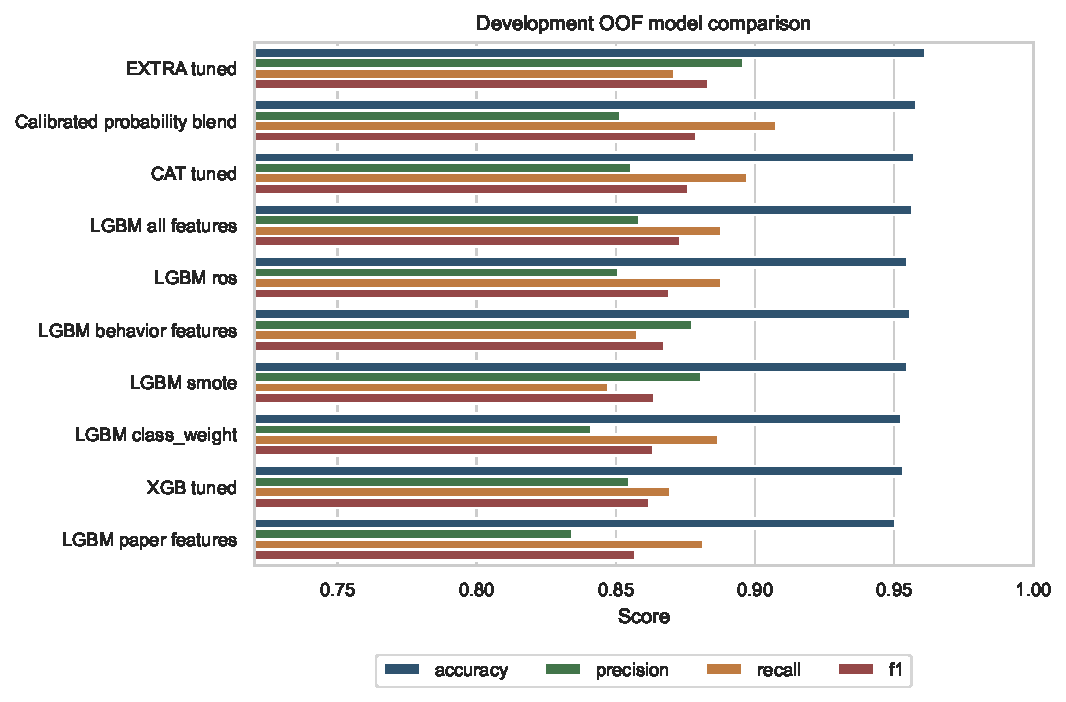
\includegraphics[width=.80\textwidth]{figures/fig04_model_comparison.pdf}\caption{Top development OOF configurations. Thresholds were selected from OOF probabilities subject to the accuracy floor.}\label{fig:models}\end{figure}

On the locked test, Extra Trees correctly classified 1,095 of 1,126 customers. It found 167 of 189 churners while issuing nine false alarms (Figure~\ref{fig:cm}). Its discrimination exceeded the matched baseline in both ROC and PR views (Figures~\ref{fig:roc} and \ref{fig:pr}). The paired customer-level bootstrap favored Extra Trees by 0.0612 F1 (95\% percentile CI 0.0326--0.0931) and 0.0230 AP (0.0112--0.0376); both intervals excluded zero (Figure~\ref{fig:ci}). These intervals quantify prediction-paired differences on this holdout, not generalization to all e-commerce populations.
\begin{figure}[H]\centering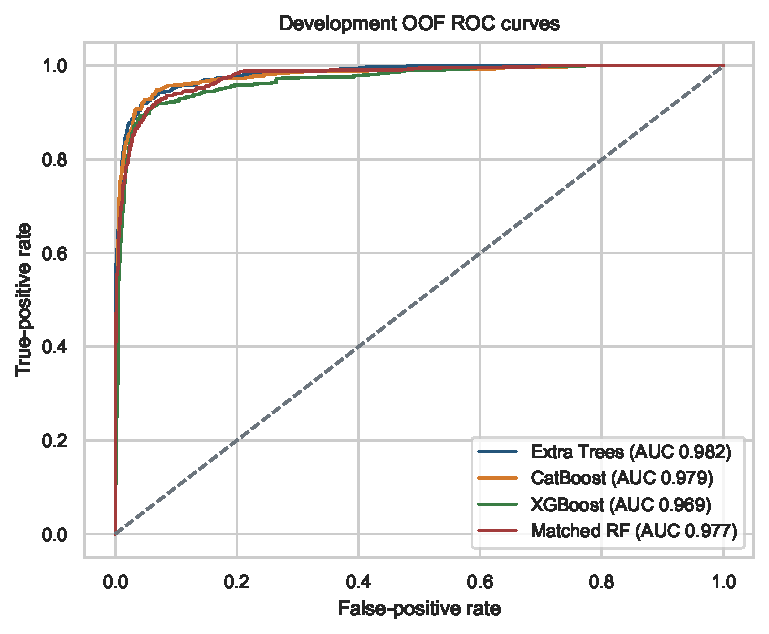
\includegraphics[width=.62\textwidth]{figures/fig05_roc_curves.pdf}\caption{Development OOF ROC curves from saved probabilities.}\label{fig:roc}\end{figure}
\begin{figure}[H]\centering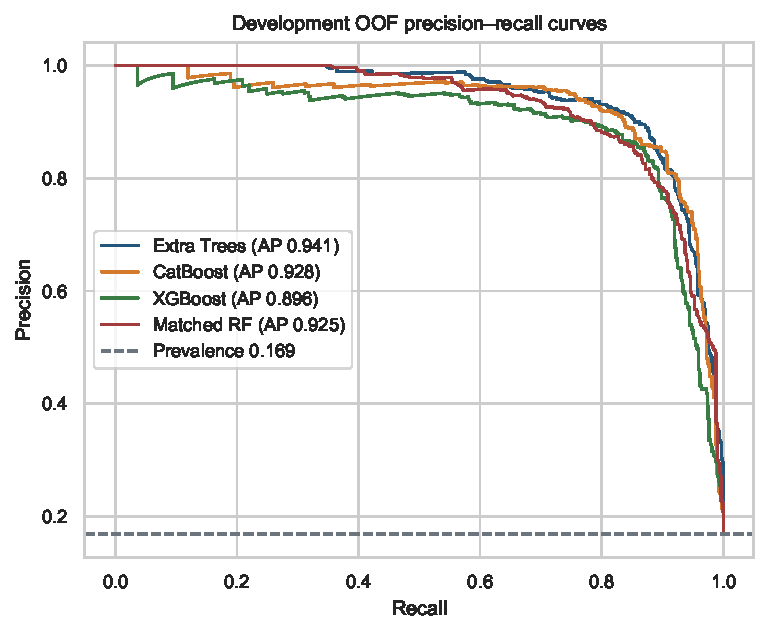
\includegraphics[width=.62\textwidth]{figures/fig06_pr_curves.pdf}\caption{Development OOF precision--recall curves.}\label{fig:pr}\end{figure}
\begin{figure}[H]\centering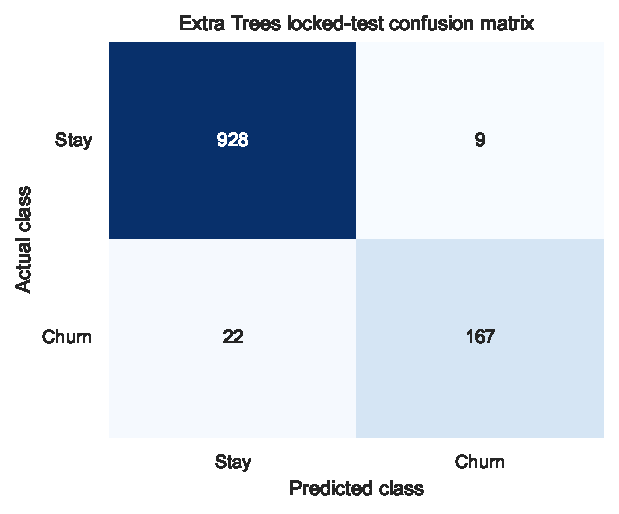
\includegraphics[width=.52\textwidth]{figures/fig07_confusion_matrix.pdf}\caption{Locked-test confusion matrix for Extra Trees.}\label{fig:cm}\end{figure}
\begin{figure}[H]\centering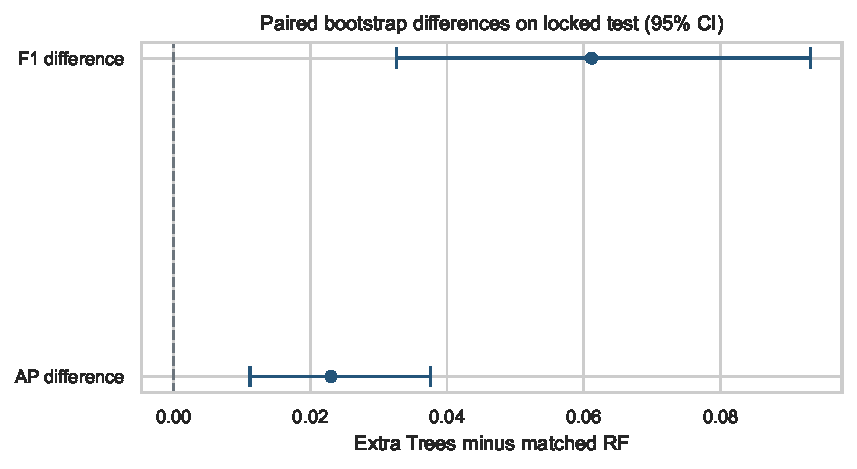
\includegraphics[width=.62\textwidth]{figures/fig12_paired_bootstrap.pdf}\caption{Paired bootstrap improvements over the matched RF.}\label{fig:ci}\end{figure}

\subsection{Ablations, calibration, and thresholding}
The paper feature alone did not improve LightGBM F1 (0.8571), and the larger behavioral feature set reached 0.8674. LightGBM with random oversampling reached 0.8691, whereas SMOTE and class weighting were slightly lower. The model-based selector reached 0.8499. The historical-style 12-feature RF reached 0.8541 OOF F1. Thus the main gain was attributable to learner choice, not engineered ratios, aggressive balancing, or reduced feature count (Figure~\ref{fig:ablation}).

Sigmoid and isotonic calibration reduced OOF AP from the uncalibrated Extra Trees result and produced F1 of 0.8702 and 0.8740, respectively. They were retained as negative experiments. The threshold curve in Figure~\ref{fig:threshold} separates operating-point effects from discrimination: changing $t$ moves accuracy, recall, and F1 but cannot change AP or ROC-AUC. Random-search traces (Figure~\ref{fig:search}) document bounded optimization rather than an exhaustive claim.
\begin{figure}[H]\centering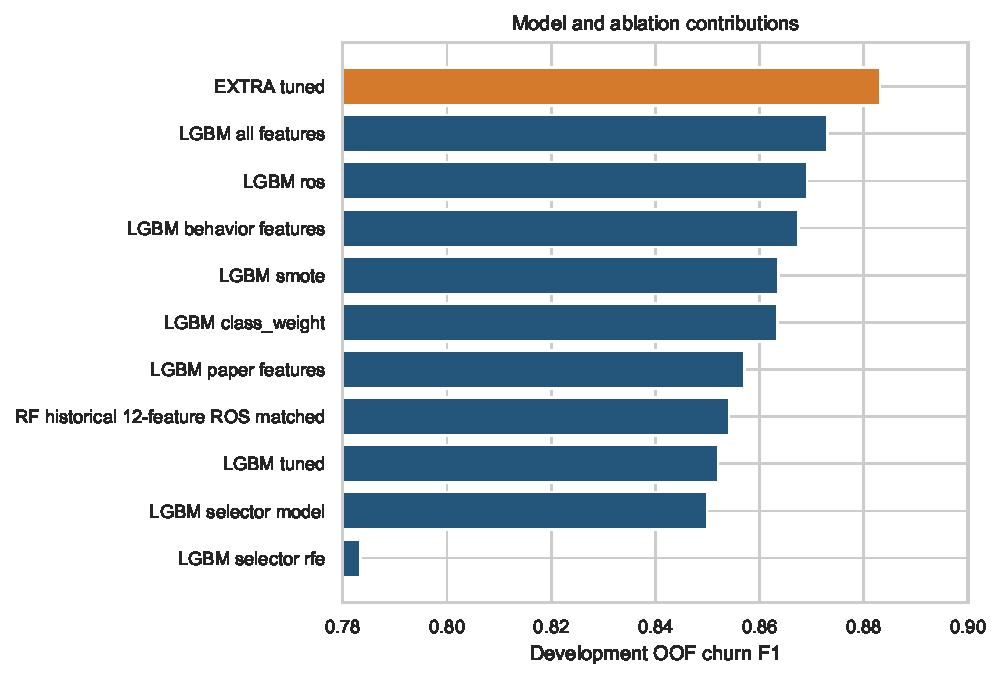
\includegraphics[width=.72\textwidth]{figures/fig09_ablation.pdf}\caption{OOF F1 for controlled learner, feature, selection, and imbalance variants.}\label{fig:ablation}\end{figure}
\begin{figure}[H]\centering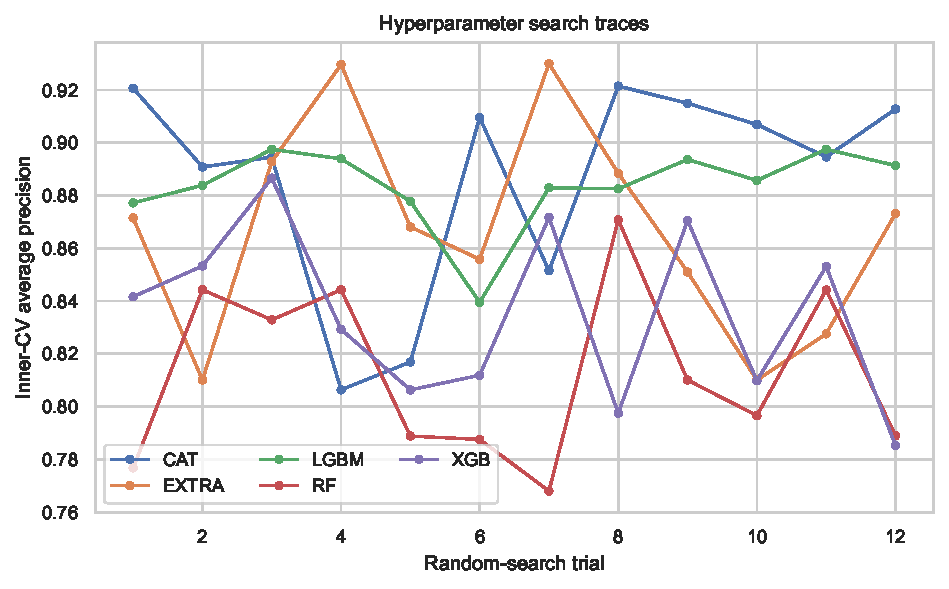
\includegraphics[width=.68\textwidth]{figures/fig10_hyperparameter_search.pdf}\caption{Inner grouped-CV search traces for five strong learners.}\label{fig:search}\end{figure}
\begin{figure}[H]\centering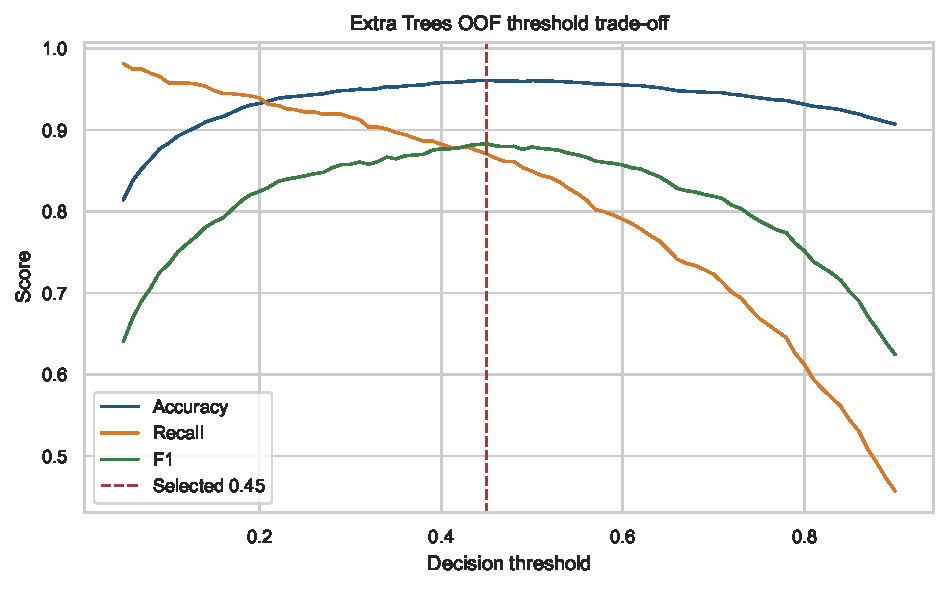
\includegraphics[width=.68\textwidth]{figures/fig11_threshold_tradeoff.pdf}\caption{Extra Trees operating-point trade-off.}\label{fig:threshold}\end{figure}
\begin{figure}[H]\centering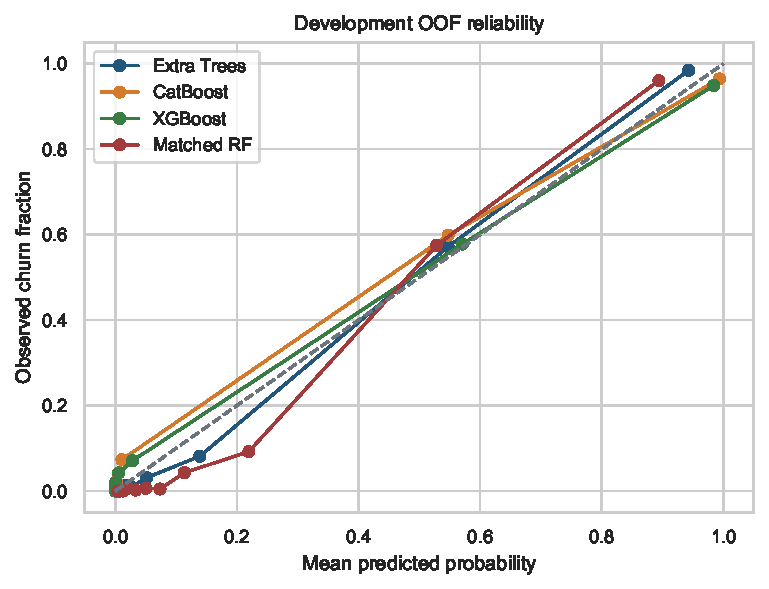
\includegraphics[width=.64\textwidth]{figures/fig13_calibration.pdf}\caption{OOF reliability curves. Calibration quality is distinct from ranking performance.}\label{fig:cal}\end{figure}

\subsection{Comparison with Sun (2025)}
Sun reported logistic regression at 0.7673 accuracy and 0.5355 F1, decision tree at 0.9432 accuracy and 0.8400 F1, and XGBoost with SMOTE and Tenure Per Device at 0.9343 accuracy, 0.8053 F1, and 0.9667 ROC-AUC \cite{sun2025churn}. Extra Trees' locked-test values are numerically higher. This is not a controlled superiority claim: the paper reports 5,629 records, does not establish the same profile-group split, and used a different modeling protocol. The valid superiority statement in this study concerns only Extra Trees versus the locally executed matched RF on identical customers.

\section{Explainable Feature Analysis}
Permutation importance was computed on development data using AP loss. Figure~\ref{fig:importance} shows the strongest variables. Importance measures predictive association after model fitting; correlated variables can share or mask importance, and no bar demonstrates that changing a customer attribute would cause retention. The unselected interaction features further caution against converting plausible business stories into unsupported model claims.
\begin{figure}[H]\centering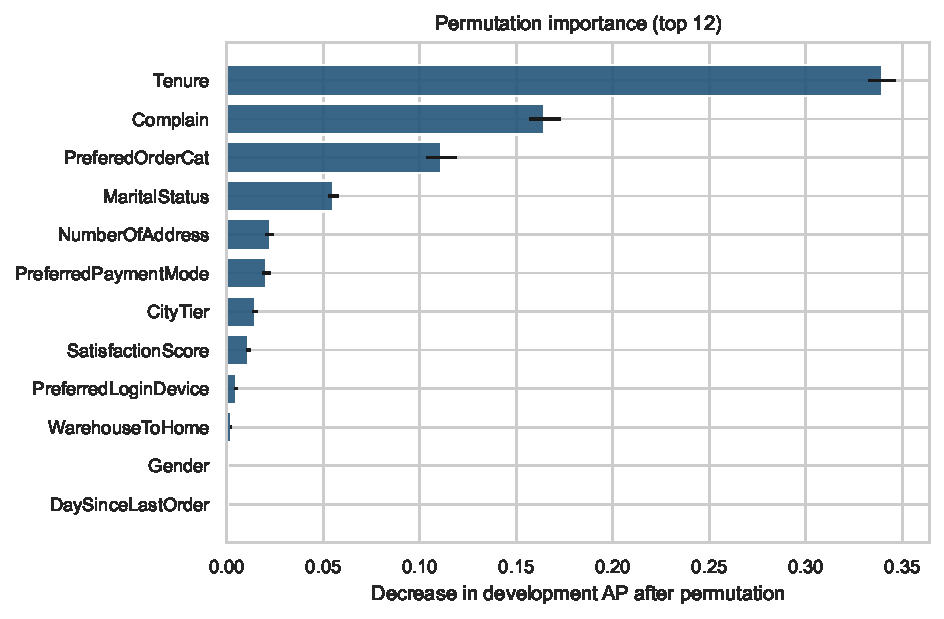
\includegraphics[width=.72\textwidth]{figures/fig08_feature_importance.pdf}\caption{Permutation importance with eight-repeat variability.}\label{fig:importance}\end{figure}

\section{Discussion}
Extra Trees improved both majority-sensitive and churn-sensitive outcomes: relative to the matched RF it added 17 true negatives and seven true positives while reducing false positives from 26 to nine and false negatives from 29 to 22. This joint movement explains the simultaneous gains in accuracy, recall, precision, F1, and AP. The result is consistent with the method's stronger randomization reducing correlation among trees \cite{geurts2006extra}, but one dataset cannot establish a universal algorithm ranking.

The probability blend represents a useful high-recall alternative: its OOF recall was 0.9078, compared with 0.8709 for Extra Trees, while its precision and F1 were slightly lower. Operationally, organizations with a low contact cost or high missed-churn cost may prefer this configuration. At top-$K$, the supplied contact table reports precision and recall for 5\%, 10\%, and 20\% targeting; these are predictive yield estimates, not causal retention uplift. Campaign value still requires randomized intervention evidence.

The analysis also illustrates why single-metric optimization is hazardous. The historical workbook's RF score is strong, yet its original test was already visible, preventing it from serving as a pristine future test for iterative research. We therefore created one predeclared group holdout and reported the old score separately. The paired improvement on the new holdout is compelling within this protocol, while external validity remains unresolved.

\section{Limitations and Future Work}
The source is a cross-sectional customer snapshot, not a chronological transaction sequence. Temporal leakage cannot be fully audited because the lineage of the globally cleaned workbook is unavailable; cleaning may have occurred before splitting. The original raw \texttt{E Commerce Dataset.xlsx} was not present, so a raw-source split-first sensitivity analysis was blocked. The paper's 5,629 rows differ by one from the workbook. Repeated profiles may reflect preprocessing or copied records, although grouping prevents cross-partition duplication.

The locked test contains only 189 churners, and the bootstrap reuses this empirical population. No independent company, period, or geography was available. Hyperparameter search was deliberately bounded to 12 trials per strong learner. Native CatBoost categorical handling was not used because a common preprocessing representation was maintained. Permutation importance is global and associational; SHAP was not required for the selected scientific claim. Future work should use raw timestamped events, rolling-origin validation, independent cohorts, cost-sensitive decision analysis, fairness assessment where lawful demographic context exists, and randomized retention interventions.

\section{Conclusion}
A leakage-aware, group-preserving comparison selected an 18-predictor Extra Trees model at threshold 0.45. It achieved 0.9725 accuracy, 0.9489 precision, 0.8836 recall, 0.9151 F1, 0.9747 AP, and 0.9938 ROC-AUC on a once-evaluated group holdout. Paired bootstrap differences over the newly executed 12-feature oversampled RF excluded zero for both F1 and AP. Feature engineering, calibration, selection, and balancing experiments were informative but did not create the winning recipe. These findings support Extra Trees as the balanced recommendation for this dataset and protocol, while cross-paper and cross-population superiority remain unproven.

\begin{thebibliography}{9}
\bibitem{breiman2001rf} L. Breiman. Random Forests. \emph{Machine Learning}, 45:5--32, 2001. doi:10.1023/A:1010933404324.
\bibitem{geurts2006extra} P. Geurts, D. Ernst, and L. Wehenkel. Extremely randomized trees. \emph{Machine Learning}, 63:3--42, 2006. doi:10.1007/s10994-006-6226-1.
\bibitem{chen2016xgb} T. Chen and C. Guestrin. XGBoost: A Scalable Tree Boosting System. In \emph{KDD}, pages 785--794, 2016. doi:10.1145/2939672.2939785.
\bibitem{ke2017lgbm} G. Ke et al. LightGBM: A Highly Efficient Gradient Boosting Decision Tree. In \emph{NeurIPS 30}, 2017.
\bibitem{prokhorenkova2018cat} L. Prokhorenkova et al. CatBoost: unbiased boosting with categorical features. In \emph{NeurIPS 31}, 2018.
\bibitem{chawla2002smote} N. V. Chawla et al. SMOTE: Synthetic Minority Over-sampling Technique. \emph{JAIR}, 16:321--357, 2002. doi:10.1613/jair.953.
\bibitem{lundberg2017shap} S. M. Lundberg and S.-I. Lee. A Unified Approach to Interpreting Model Predictions. In \emph{NeurIPS 30}, 2017.
\bibitem{niculescu2005calibration} A. Niculescu-Mizil and R. Caruana. Predicting Good Probabilities with Supervised Learning. In \emph{ICML}, pages 625--632, 2005. doi:10.1145/1102351.1102430.
\bibitem{sun2025churn} R. Sun. Customer Churn Prediction in E-Commerce Using Machine Learning Models for Digital Marketing Trends. In \emph{BDEIM 2025}, 2025. doi:10.1145/3800000.3800153.
\end{thebibliography}
\end{document}
